\documentclass[conference]{IEEEtran}
\IEEEoverridecommandlockouts
\usepackage{cite}
\usepackage{amsmath,amssymb,amsfonts}
\usepackage{algorithm}
\usepackage{algpseudocode}
\usepackage{graphicx}
\usepackage{textcomp}
\usepackage{xcolor}
\usepackage{hyperref}
\def\BibTeX{{\rm B\kern-.05em{\sc i\kern-.025em b}\kern-.08em
    T\kern-.1667em\lower.7ex\hbox{E}\kern-.125emX}}

\begin{document}

\title{A simple approach to parallelize the C4.5 algorithm for generating decision trees}

\author{\IEEEauthorblockN{Diego Henrique Oliveira}
\IEEEauthorblockA{\textit{Departamento de Informática e Estatística (INE)} \\
\textit{Universidade Federal de Santa Catarina}\\
Florianópolis, Brazil \\
diego.h.oliveira@posgrad.ufsc.br}
}

\maketitle

\begin{abstract}
TODO
\end{abstract}

\section{Introduction}

A decision tree is a simple representation for classification problems, figure \ref{fig:dtree} illustrates a decision tree that allows comparing the sample attributes with the tree nodes until they reach a leaf. The leaf is the classification of that sample in that tree. Generating a decision tree is a supervised machine learning method that analyzes a training set for which the class labels are known. The output of this method is a tree where:

\begin{itemize}
    \item \textbf{Node}: tests for the value of a particular attribute.
    \item \textbf{Branch}: corresponds to the outcome of a test and connects to the next node or leaf.
    \item \textbf{Leaf}: terminal nodes that predict the outcome.
\end{itemize}

Once generated, the decision tree can classify unforeseen samples with high confidence. According to \cite{sezer}, using a decision tree to predict maintenance has an average accuracy of 81\% to predict when a machine will exceed a quality threshold. In the proposed framework for a low-cost, easy-to-develop Cyber-Physical System that aims to predict other equipment maintenance, \cite{sezer}'s machine learning technique is Decision Trees.

\begin{figure}[h]
    \centering
    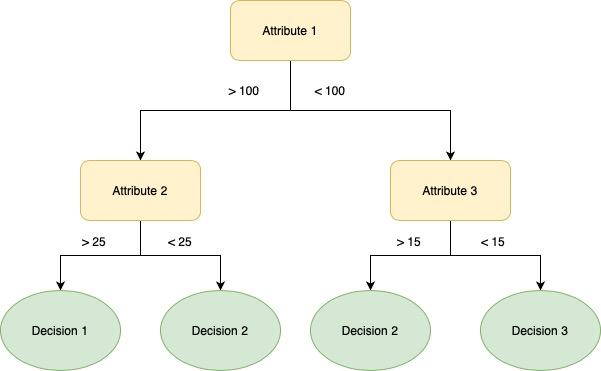
\includegraphics[width=0.8\linewidth]{images/decision-trees.jpg}
    \caption{An illustration of a decision tree}
    \label{fig:dtree}
\end{figure}

Decision trees are built using a heuristic called recursive partitioning. This approach is also commonly known as divide and conquer. It splits the data into subsets, which are then split repeatedly into even smaller subsets until the process stops when the algorithm determines that data within the subsets are sufficiently homogeneous, or another stopping criterion has been achieved. A generic, divide and conquer algorithm for generating a decision tree would be:

\begin{enumerate}
    \item Select a test for root node. Create a branch for each possible outcome of the test.
    \item Split instances into subsets, one for each branch extending from the node.
    \item Repeat recursively for each branch, using only instances that reach the branch.
    \item Stop recursion for a branch if all its instances have the same class.
\end{enumerate}

This work proposes parallelizing the C4.5 algorithm to generate a decision tree that could predict machine maintenance. The training set contains samples of the machine state over one year, available at \cite{data}. It has been used by \cite{birgelen} to build a self-organizing map, another machine learning technique, to predict the state of components of a cyber-physical system.

\section{An overview of C4.5 Algorithm}

C4.5 is a decision tree generating algorithm introduced by \cite{quinlan} as a top-down, divide and conquer algorithm that builds a decision tree picking the best attribute at each node according to the highest gain ratio. The formula \eqref{eqgain} calculates the gain ratio. The C4.5 extends the ID3 algorithm, developed by the same author, with several improvements to enhance the ID3 algorithm. According to \cite{quinlan}, some of these are:

\begin{itemize}
    \item Choosing an appropriate attribute selection measure.
    \item Handling training data with missing attribute values.
    \item Handling attributes with differing costs.
    \item Pruning the decision tree after its creation.
    \item Handling continuous attributes.
\end{itemize}

\begin{equation}
Gain(ts, a) = Entropy(ts) - \sum_{i=1}^{n} \frac{ts_i}{ts} * Entropy(ts_i) \label{eqgain}
\end{equation}

In plain English, the C4.5 algorithm can be described as the following steps:
\begin{enumerate}
    \item Let T be the set of training instances
    \item Choose an attribute that best differentiates the instances contained in T using the formula \eqref{eqgain}
    \item Create a tree node whose value is the chosen attribute
    \begin{enumerate}
        \item Create child links from this node where each link represents a unique value for the chosen attribute
        \item Use the child link values to subdivide the instances into subclasses further
    \end{enumerate}
\end{enumerate}

\section{The proposed strategy to parallelize C4.5}

Algorithm \ref{c45} contains the proposed implementation of C4.5, which has a time complexity of $O(m * n^2)$, where \textit{m} is the size of the training set, and \textit{n} is the number of attributes. The proposal of this paper is not to parallelize the complete algorithm. Instead, the focus is to parallelize the most expensive part: choosing the best attribute for a given node. 

\begin{algorithm}
\begin{algorithmic}[1]
\Procedure{C45}{$ts, attributes, class\_attr$}
    \State $best,values \gets best\_fn(ts, attributes, class\_attr)$
    
    \If{best is None}
        \State \textbf{return} $None$
    \EndIf
    
    \State $node \gets create\_node(best, len(ts))$
    
    \For{value in values}
        \State $sub\_ts \gets filter\_ts(ts, best, value)$
        \State $dist \gets create\_distribution(class\_attr, ts)$
        
        \If{is\_leaf(sub\_ts, attributes, dist)}
            \State $node.set\_as\_leaf(value, dist)$
        \Else
            \State $sub\_attr \gets filter\_attr(attributes, best)$
            \State $child \gets C45(sub\_ts, sub\_attr, class\_attr)$
            \If{child}
                \State $node.create\_branch(value, child)$
            \EndIf
        \EndIf
        
    \EndFor
   \State \textbf{return} $node$
\EndProcedure
\end{algorithmic}
\caption{The proposed C4.5 implementation}
\label{c45}
\end{algorithm}

The most expensive part of the algorithm \ref{c45} is the \textit{best\_fn}. The algorithm \ref{best_fn} describes the \textit{best\_fn} function. Here it would loop over all attributes calling the \textit{gain} function for each attribute. The \textit{gain} function would loop over the training set to calculate the gain ratio for the current attribute. The root node has the worst cost because the available attributes are all attributes of the training instance. At each level of the tree, the available attributes will be less and less, as shown in table \ref{table:attributes_len}.

\begin{table}[!ht]
\centering
\begin{tabular}{ |c|c|c|c|c| }
\hline
Tree Level &Available Attributes \\
\hline
root &n \\
level 1 &n-1 \\
level 2 &n-2 \\
level 3 &n-3 \\
leaf &n-4 \\
\hline
\end{tabular}
\caption{Number of attributes by tree level}
\label{table:attributes_len}
\end{table}


\begin{algorithm}
\begin{algorithmic}[1]
\Procedure{best\_fn}{$ts, attributes, class\_attr$}
    \State $best \gets None$
    \State $value \gets -1e999999$\Comment{The lowest float available}
    \For{attr in attributes}
        \If{attr == class\_attr}
            \State \textbf{continue}
        \EndIf
        \State $v \gets gain(ts, attr, class\_attr)$
        \If{$v > value$}
            \State $value \gets v$
            \State $best \gets attr$
        \EndIf
    \EndFor
    \State \textbf{return} $best, unique\_values(ts, best)$
\EndProcedure
\end{algorithmic}
\caption{The best\_fn implementation}
\label{best_fn}
\end{algorithm}

Our proposal is straightforward: parallelize the gain ratio calculation for each attribute. An advantage of this design is that all the gain function input is read-only, so there is no need to control the memory access to avoid race conditions. Calling the \textit{gain} function in parallel would not change the algorithm \ref{c45}, but it will involve some changes to the algorithm \ref{eqgain}. However, those changes would vary based on the programming language used since each one has its parallelism mechanism. For example, \textit{Python} has the \textit{multiprocessing} package, while \textit{Go} implements \textit{goroutines}, a lightweight thread managed by the Go \textit{runtime}. One disadvantage of this design is that the root node and the nodes close to it would have almost all parallelization benefits because the \textit{best\_fn} will have more attributes to choose from the first levels, as shown in table \ref{table:attributes_len}.

\subsection{Obtained Results}

To validate if the proposed technique would benefit the execution time of the C4.5 algorithm proposed, two implementations of the algorithm c45 were executed in a \textit{c5.4xlarge} instance of AWS EC2. As described in \cite{aws}, this instance type is optimized for compute-intensive workloads and uses 16 \textit{virtual CPUs\(vCPU\)}, powered by the AWS Nitro System \cite{aws-nitro}, a combination of dedicated hardware and \textit{lightweight hypervisor}. The training set used to run both implementations comprises 1.062.912 samples, available at \cite{data}, and each sample has six attributes. Both implementations are available at \url{https://github.com/diegoholiveira/parallel-c4.5}.

The two implementations would run in two modes: serial and parallel. The parallel version runs with 2, 4, 8, and 16 processes (16 is the total \textit{vCPU} available at the execution environment). Table \ref{table:execution_time_python} shows the execution time of the implementation in Python, using the multiprocessing package to create a pool of workers.

\begin{table}[!ht]
\centering
\begin{tabular}{ |c|c|c|c|c| }
\hline
Method &Round 1 &Round 2 &Round 3 \\
\hline
serial &1h 7m 59s &1h 0m 54s &1h 1m 10s \\
2 workers &48m 20s &48m 21s &49m 11s \\
4 workers &36m 38s &37m 9s &36m 29s \\
8 workers &36m 58s &37m 6s &36m 47s \\
16 workers &36m 56s	&37m &36m 37s \\
\hline
\end{tabular}
\caption{Time of execution of the algorithm \ref{c45} in Python 3.9}
\label{table:execution_time_python}
\end{table}

The results of the Go implementation of C45 are in table \ref{table:execution_time_go}. The technique used in this implementation is slightly different from the python implementation because of the language mechanisms of parallelization. Instead of using a pool of workers, the implementation consists and having all workers available, and the communication with these workers uses \textit{channels} to send and receive data. \textit{Channel} is a Go primitive to allow thread-safe communication between \textit{goroutines}, as described in \cite{go-channel}.

\begin{table}[!ht]
\centering
\begin{tabular}{ |c|c|c|c|c| }
\hline
Method &Round 1 &Round 2 &Round 3 \\
\hline
serial &7m &7m &7m 3s \\
2 workers &4m 17s &4m 17s &4m 18s \\
4 workers &2m 50s &2m 50s &2m 50s \\
8 workers &2m 49s &2m 50s &2m 50s \\
16 workers &2m 50s &2m 50s &2m 52s \\
\hline
\end{tabular}
\caption{Time of execution of the algorithm \ref{c45} compiled with Go 1.15}
\label{table:execution_time_go}
\end{table}

\section{Conclusion}

The obtained results indicate that this approach to parallelizing the C45 speeds up the execution of the algorithm. The gain suggests a correlation between the number of attributes and the number of workers. As we can see in figure \ref{fig:py-execution-time}, the execution time drops until the number of workers is less than the number of attributes: in the experiment executed, the sample instance contains six attributes. When the number of workers is more than the number of attributes, we stop seeing benefits in the execution time. Further works can do experiments with training sets where the instance sample comprises more attributes than the number of available \textit{vCPU}, to validate the correlation between the number of attributes and the number of workers.

\begin{figure}[h]
    \centering
    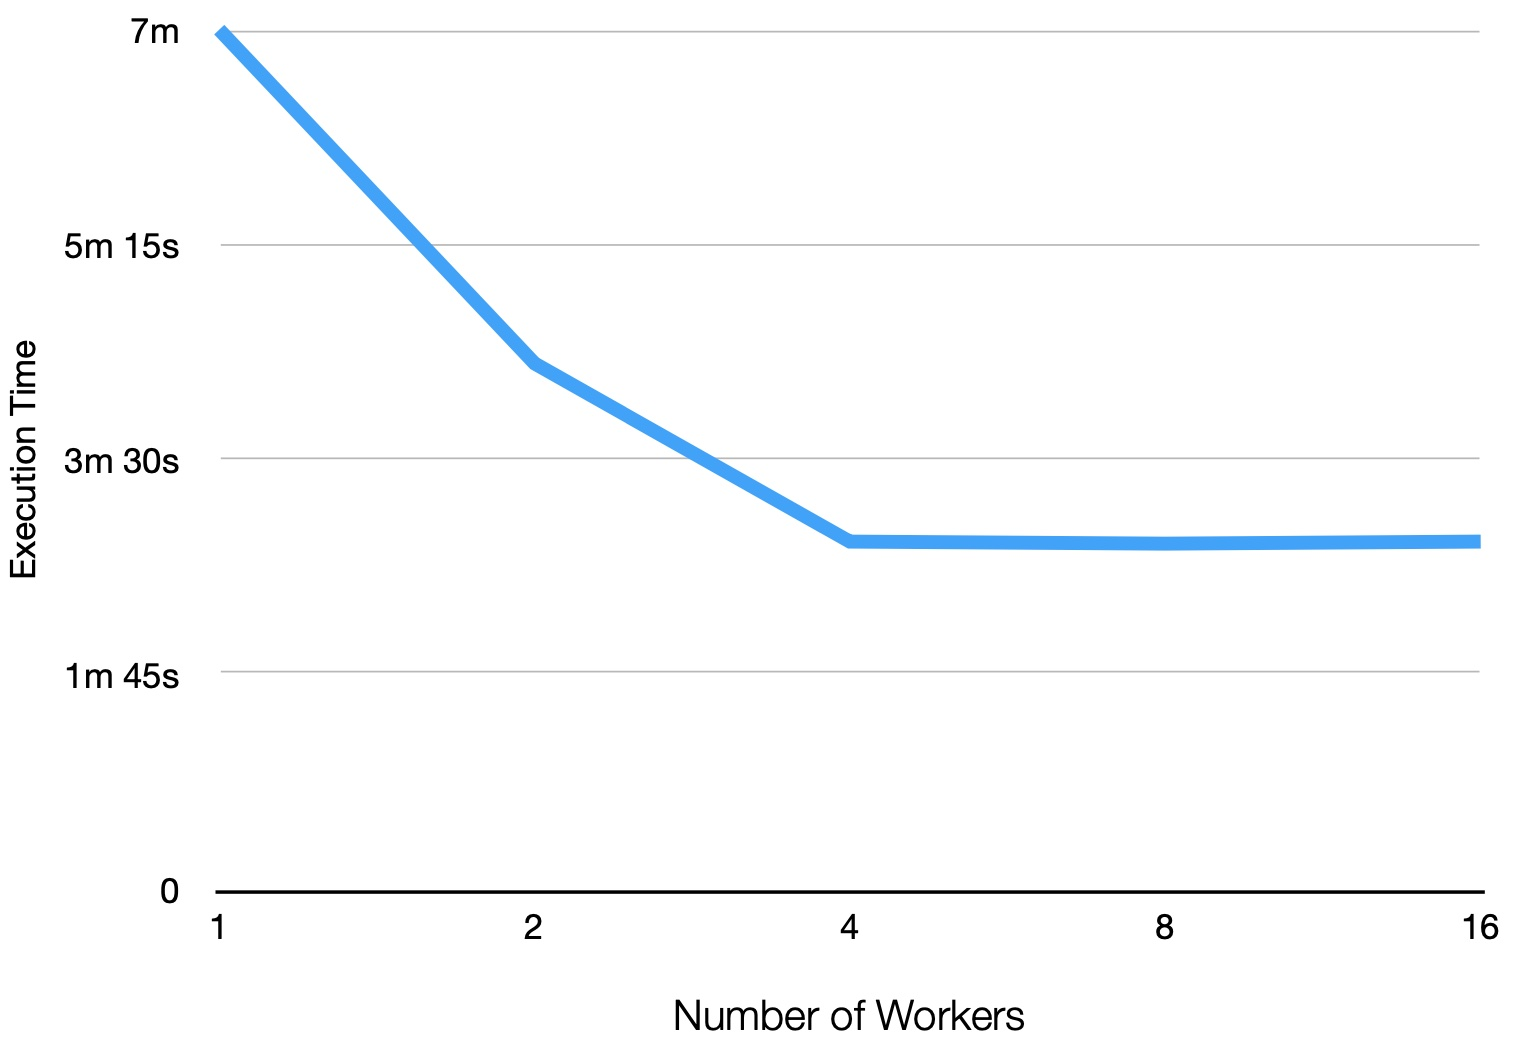
\includegraphics[width=0.8\linewidth]{images/go-execution-time.jpg}
    \caption{The execution time of the Go implementation}
    \label{fig:py-execution-time}
\end{figure}



\begin{thebibliography}{00}
\bibitem{sezer} E. Sezer, D. Romero, F. Guedea, M. Macchi, and C. Emmanouilidis, “An Industry 4.0-Enabled Low Cost Predictive Maintenance Approach for SMEs,” in 2018 IEEE International Conference on Engineering, Technology and Innovation (ICE/ITMC), Stuttgart, Jun. 2018, pp. 1–8. doi: 10.1109/ICE.2018.8436307.
\bibitem{quinlan} Quinlan, J.R, C4.5: Programs for machine learning. Morgan Kaufmann, 1992.
\bibitem{birgelen} A. von Birgelen, D. Buratti, J. Mager, and O. Niggemann, “Self-Organizing Maps for Anomaly Localization and Predictive Maintenance in Cyber-Physical Production Systems,” Procedia CIRP, vol. 72, pp. 480–485, 2018, doi: 10.1016/j.procir.2018.03.150.
\bibitem{aws} “Amazon EC2 Instance Types - Amazon Web Services,” Amazon Web Services, Inc. https://aws.amazon.com/ec2/instance-types/ (accessed Sep. 19, 2021).
\bibitem{data} “One Year Industrial Component Degradation.” https://kaggle.com/inIT-OWL/one-year-industrial-component-degradation (accessed Sep. 19, 2021).
\bibitem{aws-nitro} “AWS Nitro System,” Amazon Web Services, Inc. https://aws.amazon.com/ec2/nitro/ (accessed Sep. 19, 2021).
\bibitem{go-channel} “A Tour of Go.” https://tour.golang.org/concurrency/2 (accessed Sep. 19, 2021).

\end{thebibliography}
\end{document}
